\subsection{Installation Ubuntu WSL with Visual Studio Code}

\url{https://code.visualstudio.com/docs/cpp/config-wsl}

\begin{enumerate}
    \item Download Ubuntu 18.04 LTS from Windows Store.
    \item Activate \texttt{Windows Subsystem for Linux} through \texttt{Programs and Features}.
        \begin{figure}[H]
            \centering
            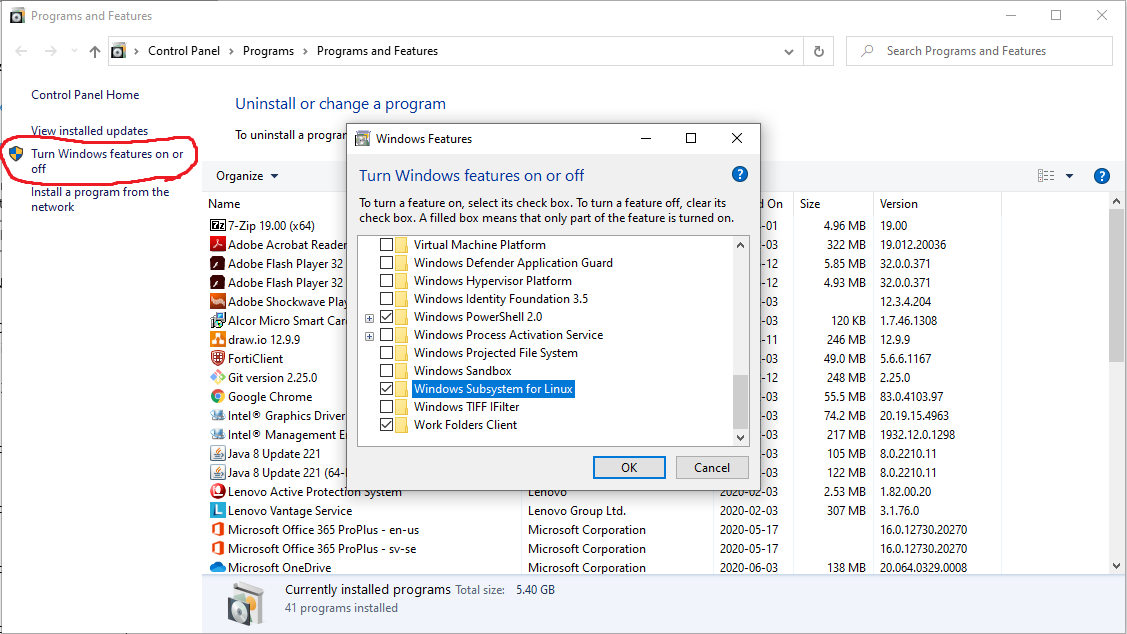
\includegraphics[width=\textwidth]{Figures/WSL/turn_on_WSL.PNG}
        \end{figure}
    \item Restart computer.
    \item Run \texttt{Ubuntu 18.04 LTS} and let it install. Might have to press \texttt{enter} after a while.
    \item Create user with password.
    \item Install \texttt{gcc} and \texttt{gdb} on the Windows Subsystem for Linux (WSL).
    \begin{enumerate}
        \item Run \code{sudo apt update}
        \item Then \code{sudo apt install build-essential} for \texttt{gcc}
        \item Then \code{sudo apt install gdb} for \texttt{gdb}
    \end{enumerate}
    \item Create a new folder in the WSL where you create a C file \texttt{helloworld.c}. New folder is necessary for Visual Studio Code to realise that there is a C compiler to setup later on as it uses the open file to do the configurations.
    \item Open up Visual Studio Code.
    \item Install two extensions in VS code:
        \begin{itemize}
            \item \texttt{C/C++} from Microsoft
            \item \texttt{Remote - WSL} from Microsoft
        \end{itemize}
    \item Press on the new icon on the left, \texttt{Remote explorer}. Right-click the \texttt{Ubuntu 18.04} and press \texttt{Connect to WSL}. A new window will appear with some connection to the WSL.
    \item Press on the extension icon the left in the new window. Press \texttt{Install in WSL: Ubuntu-18.04} button on the \texttt{C/C++} extension.
        \begin{figure}[H]
            \centering
            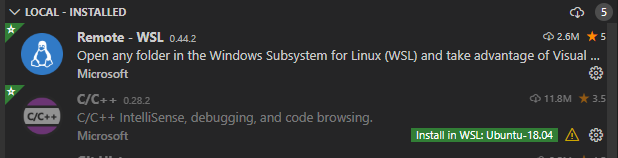
\includegraphics[width=0.7\textwidth]{Figures/WSL/vscode_extensions.PNG}
        \end{figure}
    \item By now it might prompt that you have to reload the window. Press that button.
    \item Open up the folder you created the main C file in. \texttt{File->Open Folder...}
    \item Open up the \texttt{helloworld.c} file in the file explorer.
    \item Press \texttt{Terminal->Configure Default Build Task...}. In the dropdown list that should appear, choose \code{C/C++: gcc build active file} (Not gcc-7). A file \texttt{tasks.json} will be created and opened up.
    \begin{itemize}
        \item No edits of the \texttt{tasks.json} is required for single file compilation with \texttt{gcc}.
        \item Edits are required for multi-file compilation with \texttt{gcc}.
    \end{itemize}
        \begin{figure}[H]
            \centering
            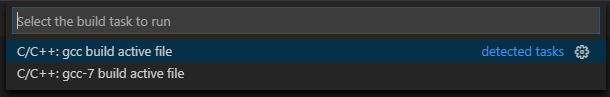
\includegraphics[width=0.7\textwidth]{Figures/WSL/vscode_compiler.PNG}
        \end{figure}
\end{enumerate}

\subsubsection{Simple single file compilation}

\begin{enumerate}
    \setcounter{enumi}{15}
    
    \item Do not edit the \texttt{tasks.json}
    
    \item Build file with \texttt{Ctrl+Shift+b}. Press the \texttt{+} sign at the terminal to open a new terminal. Run the file \code{./helloworld} to test that everything is working.
    
    \item Now onto debugging. Press \texttt{F5} or \texttt{Run->Start Debugging}. In the drop-down list that should appear, choose \code{C++ (GDB/LLDB)}. A file \texttt{launch.json} will be created and opened up.
    
        \begin{figure}[H]
            \centering
            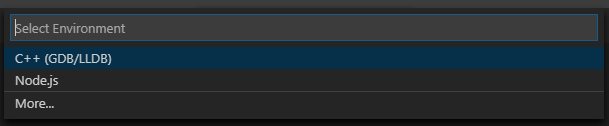
\includegraphics[width=0.7\textwidth]{Figures/WSL/vscode_environment_c++.PNG}
        \end{figure}
        
    \item Do not edit the \texttt{launch.json}.
    
    \item Down at the \texttt{Output} and \texttt{Terminal}, press the three dots \texttt{...} and choose \texttt{Debug Console} in which one can run the standard \texttt{gdb} commands.
    
\end{enumerate}

\subsubsection{Multi-file compilation with Makefile}

Here is an example of a \texttt{Makefile} I have used. Rembemer to use the \code{-g} flag if you want to debug. Also available here \url{https://github.com/robinhellmers/computer_setup}.

This \texttt{Makefile} is based on the following structure.
\begin{itemize}
    \item \texttt{Makefile} in the main project folder.
    \item Four sub-folders: \texttt{bin}, \texttt{src}, \texttt{include}, \texttt{lib}
    \item Executable \texttt{.out} files in \texttt{bin}.
    \item Main \texttt{.c} files in \texttt{src}.
    \item Extra \texttt{.c} used as libraries in \texttt{lib}.
    \item All \texttt{.h} header files in \texttt{include}.
\end{itemize}

\begin{minted}[tabsize=3,obeytabs,linenos,bgcolor=codegray]{make}
CC := gcc
CFLAGS := -pthread -g

BIN := bin
SRC := src
INCLUDE := include
LIB := lib

all: $(BIN)/server.out $(BIN)/client.out

$(BIN)/server.out: $(SRC)/server.c $(LIB)/*.c $(INCLUDE)/*.h
	$(CC) $(CFLAGS) -I$(INCLUDE) $^ -o $@

$(BIN)/client.out: $(SRC)/client.c $(LIB)/*.c $(INCLUDE)/*.h
	$(CC) $(CFLAGS) -I$(INCLUDE) $^ -o $@

clean:
	rm $(BIN)/server.out $(BIN)/client.out



# ${wildcard pattern}
# "wildcard" will list every file that follows the "pattern"
#
# Lets say we have the files hello.c hello.h goodbye.c goodbye.h
# ${wildcard *.c} will result in: hello.c goodbye.c
\end{minted}

After creating one for the specific project, continue with the \textbf{Visual Studio Code} configuration:

\begin{enumerate}
    \setcounter{enumi}{15}
    
    \item The \texttt{tasks.json} must be edited according to the following.
    
    \begin{itemize}
        \item Might have to check if there is some information in the generated \texttt{tasks.json} about the version number.
        
        \item Code also available here: \url{https://github.com/robinhellmers/computer_setup} in the \texttt{.vscode} folder.
        
        \item This edit will require a \texttt{Makefile} with an \code{make all} command for compiling all the different files together.
        
        \item The label \code{"label": "build"} can be changed to any other, which will be used in the debugger config file \texttt{launch.json} later on. Same label will appear as a dropdown list later on.
    \end{itemize}
    
\begin{minted}[tabsize=3,obeytabs,linenos,bgcolor=codegray]{json}
{
    "version": "2.0.0",
    "tasks": [
        {
            "type": "shell",
            "label": "build",
            "command": "make all",
            "group": {
                "kind": "build",
                "isDefault": true
            },
            "problemMatcher": "$gcc"
        }
    ]
}
\end{minted}
    
    \item Build file with \texttt{Ctrl+Shift+b}. Press the \texttt{+} sign at the terminal to open a new terminal. Run the file \code{./helloworld} to test that everything is working.
    
    \item Now onto debugging. Press \texttt{F5} or \texttt{Run->Start Debugging}. In the drop-down list that should appear, choose \code{C++ (GDB/LLDB)}. A file \texttt{launch.json} will be created and opened up.
    
        \begin{figure}[H]
            \centering
            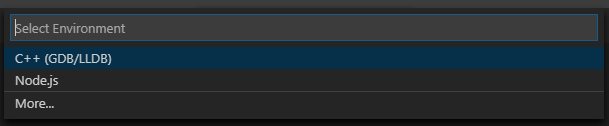
\includegraphics[width=0.7\textwidth]{Figures/WSL/vscode_environment_c++.PNG}
        \end{figure}
    
    \newpage
    \item The \texttt{launch.json} must be edited according to the following.
    \begin{itemize}
        \item Might have to check if there is some information in the generated \texttt{tasks.json} about the version number.
        
        \item Code also available here: \url{https://github.com/robinhellmers/computer_setup} in the \texttt{.vscode} folder.
        
        \item Set the prelaunch task \code{"preLaunchTask": "build"} to the label you set in the \texttt{tasks.json}, in this case to \code{"build"}. This will do the compilation according to our specification in the \texttt{tasks.json} and thereby compile with the \texttt{Makefile}.
        
        \item Set which program to debug with\\\code{"program": "\$\{workspaceFolder\}/bin/\$\{fileBasenameNoExtension\}.out"}.\\This must be adjusted according to the \texttt{Makefile} and where it saves its executable file. Remember to adjust the file ending according to what the \texttt{Makefile} outputs.
    \end{itemize}
    
\begin{minted}[tabsize=3,obeytabs,linenos,bgcolor=codegray]{json}
{
    "version": "0.2.0",
    "configurations": [
        {
            "name": "gcc - Build and debug active file",
            "type": "cppdbg",
            "request": "launch",
            "program": "${workspaceFolder}/bin/${fileBasenameNoExtension}.out",
            "args": [],
            "stopAtEntry": false,
            "cwd": "${workspaceFolder}",
            "environment": [],
            "externalConsole": false,
            "MIMode": "gdb",
            "setupCommands": [
                {
                    "description": "Enable pretty-printing for gdb",
                    "text": "-enable-pretty-printing",
                    "ignoreFailures": true
                }
            ],
            "preLaunchTask": "build",
            "miDebuggerPath": "/usr/bin/gdb",
            "sourceFileMap": {
                "/build/glibc-2ORdQG": "/usr/src/glibc"
            }
        }
    ]
}
\end{minted}

\end{enumerate}

\newpage
Now when debugging and the debugger quits the program, there will always be an error about now able to open a specific file such as \code{/build/glibc-2ORdQG} or some other letters and numbers after \code{glibc-...}. This is not a problem more than that it is annoying. This can be fixed by downloading the files which it wants to open.

\begin{enumerate}
    \setcounter{enumi}{20}
    
    \item Download \texttt{glibc} compressed file with \code{sudo apt install glibc-source}.
    
    \item Go to the right directory \code{cd /usr/src/glibc}
    
    \item Extract the content of the compressed file with \code{sudo tar xf glibc-2.27.tar.xz}
    
    \item Now add the following, except the most outer curly brackets, to the \texttt{launch.json} file under\\\code{"configurations": [\{...\}]}
    \begin{itemize}
        \item The letters and numbers after \code{glibc-...} must be adjusted to the error message that pops up when the debugger is quitting the program.
    \end{itemize}
    
\begin{minted}[tabsize=3,obeytabs,linenos,bgcolor=codegray]{json}
{
    "sourceFileMap": {
        "/build/glibc-2ORdQG": "/usr/src/glibc"
    }
}
\end{minted}

\end{enumerate}
\subsubsection{Extra}
Here is some info about setting up Visual Studio Code to build and debug projects including multiple \code{.c} files:
\begin{itemize}
    \item \url{https://dev.to/talhabalaj/setup-visual-studio-code-for-multi-file-c-projects-1jpi}
\end{itemize}

\subsubsubsection{Search for multiple words}

Some times you might want to find a specific \texttt{file} or \texttt{line of code} with multiple words in it, without having to be in a direct sequence. Use this extension which automates the process of using \texttt{regex}.

\textbf{Search} by \textbf{Alexander}:

\url{https://marketplace.visualstudio.com/items?itemName=usernamehw.search}